\documentclass[12pt,fleqn]{article}\usepackage{../../common}
\begin{document}
Momentum Stratejileri

Momentum kelimesi akılda ivmeli bir hareketi çağrıştırıyor, yani olmakta
olan bir gidişatın olmaya devam etmesi gibi görebiliriz bu kavramı. Bu tür
bir kalıcılık, yukarı ya da aşağı doğru, borsacı için al/sat bağlamında
önemli bir sinyaldir ve kar amaçlı olarak kullanılabilir. 

Araştırmacılar bazen varlık fiyatlarındaki momentumu ikiye ayırıyorlar;
zaman serisi momentumu ve kesitsel (cross-sectional) momentum. Zaman serisi
momentumu basit: bir serinin gelecekteki getirisinin geçmişteki getirisi
ile arasında pozitif korelasyon vardır. Kesitsel durumda ise izafi bir olay
vardır: eğer bir serinin getirisi diğer serilerden daha iyi olmuş ise, bu
performans büyük bir ihtimalle bu şekilde devam edecektir, ya da tersi
durumda, kötü performans kötü olmaya devam edecektir. 

Zaman serisi korelasyonunu ölçmek için istatistiki korelasyon hesabını
kullanabiliriz, ki bu hesap ayrıca bir p-değeri de hesaplıyor (korelasyon
olmadığı sıfır hipotezinin sıfır değeri), çok düşük p-değeri korelasyon
varlığına dair bir işaret.

Korelasyon hesaplarken bir zaman adımı / gecikmesi (lag) seçmek
lazım. Mesela 1 günlük bazında hesaplanmış geçmiş ve gelecek getirileri
arasında negatif korelasyon bulunabilir, ama 20 günlük adımlar üzerinden
hesaplanmış getirilerin 40 günlük adımlar üzerinden hesaplanmış gelecek
getirileri arasında pozitif korelasyon bulunabilir. Bu tabii ki önemli
çünkü bu bize 20 günlük sinyal üzerinden 40 günlük elde tutma (ya da açığa
satma) işlemi yapmamız gerektiğini söylüyor.

Örnek olarak 2 yıllık Hazine Vadeli İşlem Sözleşmesinin (Treasury Future)
fiyatını işleyelim. Bu varlığın geçmişteki ve gelecekteki farklı
kombinasyondaki adımlar üzerindeki getirilerinin korelasyonunu test
edeceğiz; mesela geçmiş getiriyi (lookback) 5 günlük adımlardan hesaplayıp,
geleceği (hold days) 10 günlük adımlardan hesaplamak gibi. Ya da 10-10,
25-60, vs, ve tüm bu farklı kombinasyonların verilerinin ikili olarak
korelasyonunu alıp onların p-değerini hesaplayacağız.

\begin{minted}[fontsize=\footnotesize]{python}
import sys; sys.path.append('../tser_draw_sharpe')
import pandas as pd
df = pd.read_csv('TU.csv')
\end{minted}

\begin{minted}[fontsize=\footnotesize]{python}
import sys; sys.path.append('../tser_coint')
import corr

res = []
for lookback in [1, 5, 10, 25, 60, 120, 250]:
   for holddays in [1, 5, 10, 25, 60, 120, 250]:
       df_Close_lookback = df.Close.shift(lookback)
       df_Close_holddays = df.Close.shift(-holddays)
       df['ret_lag'] = (df.Close-df_Close_lookback)/df_Close_lookback
       df['ret_fut'] = (df_Close_holddays-df.Close)/df.Close
       dfc = df[['ret_lag','ret_fut']].dropna()
       idx = None
       if lookback >= holddays: 
           idx = np.array(range(0,len(dfc.ret_lag), holddays))
       else: 
           idx = np.array(range(0,len(dfc.ret_lag), lookback))
       dfc = dfc.ix[idx]
       t, x, p = corr.p_corr(dfc.ret_lag, dfc.ret_fut)
       res.append([lookback, holddays,  t, p])
res = pd.DataFrame(res,columns=['geriye bakis','tutma gunu','korelasyon','p degeri'])
print res[res['geriye bakis'] >= 25]
\end{minted}

\begin{verbatim}
    geriye bakis  tutma gunu  korelasyon  p degeri
21            25           1   -0.013846  0.270625
22            25           5    0.032196  0.263327
23            25          10    0.151663  0.017386
24            25          25    0.194388  0.045128
25            25          60    0.233075  0.021371
26            25         120    0.149209  0.102255
27            25         250    0.261104  0.015751
28            60           1    0.031111  0.088828
29            60           5    0.079022  0.063314
30            60          10    0.170948  0.009661
31            60          25    0.182575  0.059741
32            60          60    0.213958  0.123890
33            60         120   -0.036387  0.424304
34            60         250    0.318615  0.049219
35           120           1    0.021126  0.187942
36           120           5    0.053784  0.157502
37           120          10    0.092116  0.112675
38           120          25    0.152030  0.104487
39           120          60   -0.023771  0.451293
40           120         120    0.217406  0.227647
41           120         250    0.403921  0.085531
42           250           1    0.040612  0.058007
43           250           5    0.105563  0.034167
44           250          10    0.178648  0.014633
45           250          25    0.273233  0.018136
46           250          60    0.319392  0.064088
47           250         120    0.354586  0.142317
48           250         250    0.512954  0.188391
\end{verbatim}

Kod bir anlamda her zaman anı için o andaki tarihsel getiri ve eğer o
noktada pozisyon alınmış olsa eldeki varlığın tutulmasından elde edilecek
getiri hesabını yapıyor. Bu iki hesaptan iki zaman serisi türetiliyor,
sonra geriye bakış, tutma günü arasından ufak olanı oranında bu seri
örnekleniyor (sample). Niye bu örnekleme? Bu lazım, çünkü geriye bakış,
alış belli aralıklardan yapılır, çok ufak (ya da hiç) örnekleme yapsak
birbiriyle çakışan hesapları üst üste görmüş olurduk.

Seçimimizi yapmak için en iyi korelasyon katsayısı ve p-değeri arasında bir
denge gözetmek gerektiğini görüyoruz, bazen iyi olabilecek bir katsayı için
p-değeri iyi olmayabiliyor.  (60, 10), (60, 25), (250, 10), (250, 25),
(250, 60), (250, 120) eşleri bu bağlamda en iyi dengede olanlar herhalde,
ve al/sat yapmaya gelince bizim genel tercihimiz düşük elde tutma gününe ve
ayrıca en yüksek Sharpe oranına sahip olan varlıklar tabii ki. Para
kazanmak için 10 gün mü 100 gün mü beklemek daha iyi? Eğer getiriler kabaca
iki tarafta eşit ise 10 gün tercihimiz!

Şimdi getiriyi hesaplayalım. Bu hesap için 250,25 kombinasyonunu seçelim,
bu kombinasyonun katsayısı 0.273233 p-değeri 0.018. Fena değil. Stratejiyi
şöyle kodlayacağız, eğer geçmişteki 12 aylık (aşağı yukarı 250 gün) getiri
pozitif ise, hisseyi alıp bu pozisyonda 1 ay (25 gün) dur. Pozitif /
negatif bize al / sat yönünde sinyal çünkü korelasyon olduğunu biliyoruz ya
artık, demek ki eskiden çıkmışsa gelecekte çıkacak, düşmüşse gelecekte
düşecek. Bu bilinen bir strateji aslında ama biz onu biraz değiştirdik,
al/sat kararını her ay vermeye çalışmak yerine her gün vereceğiz, ve her
gün alım/satım için sermayemizin 1/25'ini kullanacağız.

\begin{minted}[fontsize=\footnotesize]{python}
import dd

def report(df,lookback,holddays):

    longs = df.Close > df.Close.shift(lookback)
    shorts = df.Close < df.Close.shift(lookback)
    df['pos'] = 0.
    for h in range(holddays):
       long_lag = longs.shift(h).fillna(False)
       short_lag = shorts.shift(h).fillna(False)
       df.loc[long_lag,'pos'] += 1
       df.loc[short_lag,'pos'] -= 1

    ret=(df.pos.shift(1)* (df.Close-df.Close.shift(1)) / df.Close.shift(1)) \
         / holddays # sermayenin holddays'lik parcasini kullan

    cumret=np.cumprod(1+ret)-1

    print 'APR', ((np.prod(1.+ret))**(252./len(ret)))-1
    print 'Sharpe', np.sqrt(252.)*np.mean(ret)/np.std(ret)
    print 'Dusus Kaliciligi', dd.calculateMaxDD(np.array(cumret))
    return cumret

cumret=report(dftu,lookback = 250,holddays = 25)
\end{minted}

\begin{verbatim}
APR 0.0167080584229
Sharpe 1.04172346649
Dusus Kaliciligi (-0.024847461773700896, 343.0)
\end{verbatim}

Tabii al/sat kararlaştırınca bu al ve satların 25 gün elde tutulması ve
bunların birikmesi durumunu hesaplamak lazım, bunu da $h=0,1,..,25$ kadar
kaydırıp bu kaydırılmış 25 vektörü toplayarak elde elde ediyoruz, mesela
sadece 3 vektör için gösterelim,

\begin{verbatim}
+ + + ... - - + - ...
  + + + ... - - + - ...
    + + + ... - - + - ...
\end{verbatim}

Üstteki ilk satır al/sat kararları, arka arkaya 3 al kararı var, bunlar
toplana toplana 3. günde 3 birim varlık birikmiş olacak, aynı şekilde
satlar eksiltilir, vs. Diğer hesaplar önceden gördüğümüz tanıdık getiri,
kumulatif getiri hesapları.

\begin{minted}[fontsize=\footnotesize]{python}
plt.plot(cumret)
plt.title(u'Kümülatif Birleşik Getiri')
plt.savefig('tser_mom_01.png')
\end{minted}

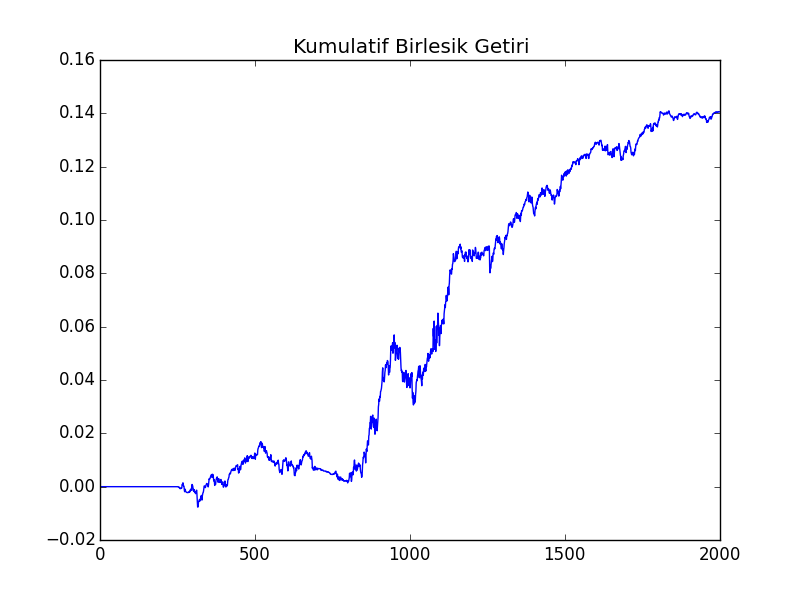
\includegraphics[height=6cm]{tser_mom_01.png}

Aynı stratejiyi diğer bazı vadeli işlemler HG, BRE üzerinde kullanırsak,

\begin{minted}[fontsize=\footnotesize]{python}
dfhg = pd.read_csv('HG.csv')
cumret = report(dfhg,lookback = 40,holddays = 40)
\end{minted}

\begin{verbatim}
APR 0.177399755457
Sharpe 1.04800326416
Dusus Kaliciligi (-0.23984679762413508, 424.0)
\end{verbatim}

\begin{minted}[fontsize=\footnotesize]{python}
plt.plot(cumret)
plt.savefig('tser_mom_04.png')
\end{minted}

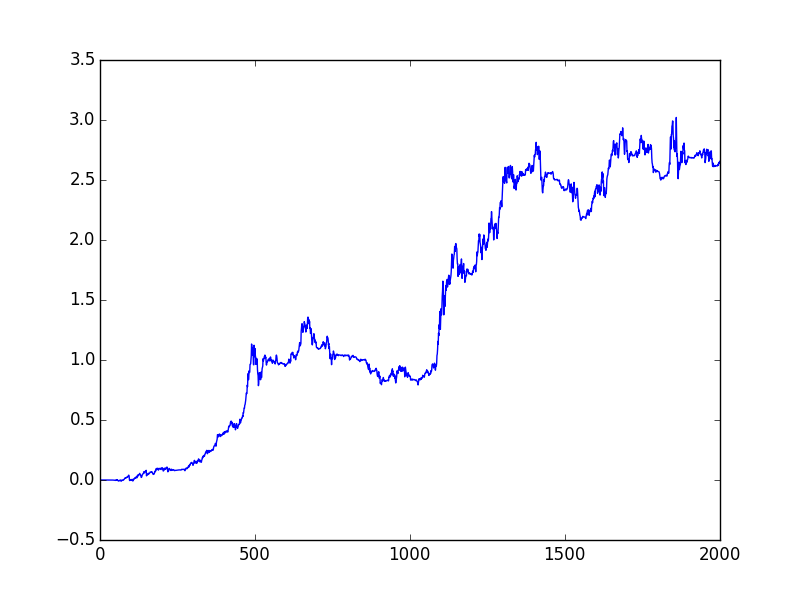
\includegraphics[height=6cm]{tser_mom_04.png}

\begin{minted}[fontsize=\footnotesize]{python}
dfbre = pd.read_csv('BRE.csv')
cumret = report(dfbre,lookback = 100,holddays = 10)
\end{minted}

\begin{verbatim}
APR 0.177086083041
Sharpe 1.08707778803
Dusus Kaliciligi (-0.14812255240727923, 191.0)
\end{verbatim}

\begin{minted}[fontsize=\footnotesize]{python}
plt.plot(cumret)
plt.savefig('tser_mom_05.png')
\end{minted}

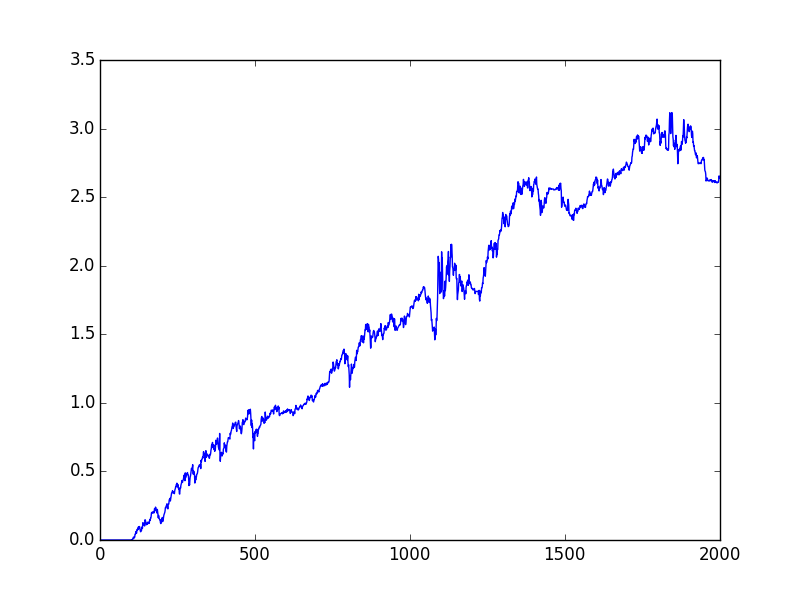
\includegraphics[height=6cm]{tser_mom_05.png}

Boşluk Görünce Alım (Buy on Gap)

Değişik bir momentum stratejisi ``boşluk görünce işlem yapmak''. Mesela bir
varlığın kapanış (close) getirilerini bir pencere üzerinden yürüyen
ortalamayla (moving average) hesaplıyoruz, böylece bir baz şablon
oluşturuyoruz, eğer bir günün açılış (open) fiyatı bu şablon getiri, çarpı
önceki günün en yüksek (high) fiyatından belli oranda yüksek ise alım
yapıyoruz, önceki günün en düşük (low) fiyatından belli oranda düşük ise
satım yapıyoruz. Yani yükselme trendi var, bir momentum oluşmuş, bu devam
ediyor, bu alım sinyalidir, ya da tersi olmuştur bu satış sinyalidir.

Altta FSTX sembolüne sahip Dow Jones STOXX 50 vadeli işlem sözleşmesinin
(futures) üzerinde bu tekniği görebiliriz,

\begin{minted}[fontsize=\footnotesize]{python}
import pandas as pd, dd
df = pd.read_csv('FSTX.csv')
entryZscore=0.1

stdret = pd.rolling_mean(df.cl.pct_change(), window=90).shift(1)
longs = df.op >= df.hi.shift(1)*(1+entryZscore*stdret)
shorts = df.op <= df.lo.shift(1)*(1-entryZscore*stdret)
df['pos'] = 0
df.loc[longs,'pos'] = 1
df.loc[shorts,'pos'] = -1
ret=df.pos * (df.op-df.cl) / df.op
ret = ret.dropna()
cumret=np.cumprod(1+ret)-1
print 'APR', ((np.prod(1.+ret))**(252./len(ret)))-1
print 'Sharpe', np.sqrt(252.)*np.mean(ret)/np.std(ret)
print 'Dusus Kaliciligi', dd.calculateMaxDD(np.array(cumret))
\end{minted}

\begin{verbatim}
APR 0.140771737387
Sharpe 1.35989260747
Dusus Kaliciligi (-0.14880173773680128, 190.0)
\end{verbatim}

\begin{minted}[fontsize=\footnotesize]{python}
plt.plot(cumret)
plt.title(u'Kümülatif Birleşik Getiri')
plt.savefig('tser_mom_02.png')
\end{minted}

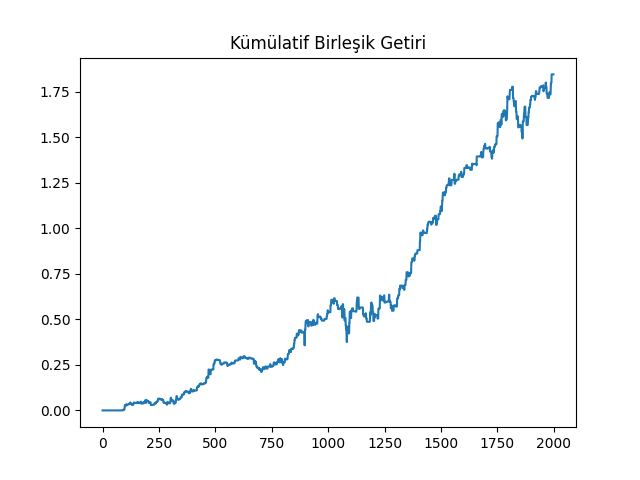
\includegraphics[height=6cm]{tser_mom_02.png}

Şirket Kar Açıklamaları

Kar açıklamalarının şirket fiyatlarına momentum vermesi şaşırtıcı
değil. Fakat bu açıklamanın ardından nispeten uzun bir süre bu
etkinin sürmesi ilginç. Daha ilginç olan bu etki uzun süredir biliniyor ve
kullanıla kullanıla etkisi yokolabilirdi, fakat bu hala gerçekleşmedi! 

Kâr açıklamalarını kullanan strateji çok basit: açıklamanın ``iyi'' ya da
``kötü'' olduğunu bile bilmemize gerek yok, o sinyali almak için yine
piyasanın kendisini kullanacağız. Eğer önceki gün kapanış sonrası bir
açıklama yapılmışsa, ve yine önceki günün kapanışı ve bugünin açılışı
üzerinden hesaplanan getiri ``yeterince'' pozitif ise (ki bunu hareketli
standart sapmaya izafi olarak hesaplayacağız), senedi al, yoksa açığa sat,
ve günün kapanışında tüm pozisyonlardan çık. Burada yapmaya uğraştığımız
momentumu, bir senet etrafında olan ``heyecanı'' açılışın önceki günün
kapanışına göre farkından anlamaya çalışmak.

Altta bu stratejinin S\&P 500 senetleri üzerinde ve Ocak 3, 2011, to Nisan
24, 2012 arasında geriye dönük testini görüyoruz. Şirket kar açıklamaları,
açılış, kapanış fiyatları farklı matrisler içinde. Her matrisin
kolonlarında şirketler var, satırları ise zaman. Geriye bakış zamanı 90
gün. Kar açıklama verisi \url{earnings.com} sitesinden alınmış.

\begin{minted}[fontsize=\footnotesize]{python}
import pandas as pd, zipfile, dd
with zipfile.ZipFile('earnann.zip', 'r') as z:
    earnann =  pd.read_csv(z.open('earnann.csv'),sep=',')
    op =  pd.read_csv(z.open('earnann-op.csv'),sep=',')
    cl =  pd.read_csv(z.open('earnann-cl.csv'),sep=',')
\end{minted}

\begin{minted}[fontsize=\footnotesize]{python}
lookback=90
retC2O=(op-cl.shift(1)) / cl.shift(1)
stdC2O=pd.rolling_std(retC2O, window=lookback)
pos = pd.DataFrame(np.zeros(cl.shape),index=cl.index,columns=cl.columns)
longs=(retC2O >= 0.5*stdC2O).astype(int) * earnann
shorts=(retC2O <= -0.5*stdC2O).astype(int) * earnann;
pos = pos + longs - shorts
ret=(pos*(cl-op)/op).sum(axis=1)/30.

cumret=np.cumprod(1+ret)-1
print 'APR', ((np.prod(1.+ret))**(252./len(ret)))-1
print 'Sharpe', np.sqrt(252.)*np.mean(ret)/np.std(ret)
print 'Dusus Kaliciligi', dd.calculateMaxDD(np.array(cumret))
\end{minted}

\begin{verbatim}
APR 0.0681264455203
Sharpe 1.49474260654
Dusus Kaliciligi (-0.026051533343801503, 109.0)
\end{verbatim}

Üstteki hesapta 30'a böldük çünkü bir günde aşağı yukarı bu kadar kar
açıklaması yapılıyor, 

\begin{minted}[fontsize=\footnotesize]{python}
print earnann.sum(axis=1).max()
\end{minted}

\begin{verbatim}
41
\end{verbatim}

\begin{minted}[fontsize=\footnotesize]{python}
plt.plot(cumret)
plt.title(u'Kümülatif Birleşik Getiri')
plt.savefig('tser_mom_03.png')
\end{minted}

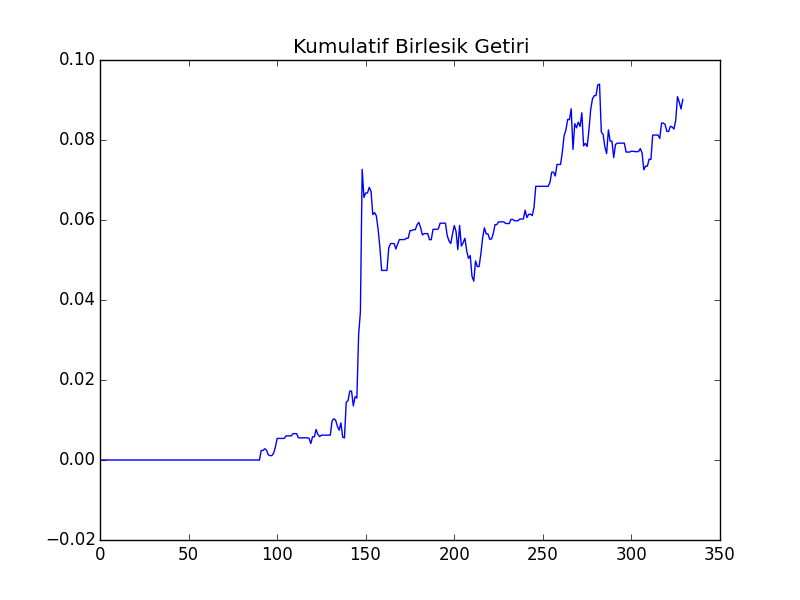
\includegraphics[height=6cm]{tser_mom_03.png}

Üstel Yürüyen Ortalama (EWMA) ile Momentum 

Pandas'in EWMA hesabı için bir çağrısı var, olağan durumunda üstelli
katsayıları kullanır, fakat istenirse özyineli formda da hesap yapabilir. 
Pandas ile pencere gibi bir parametre var, buna kapsam (span)
deniyor. Kapsam $k$ ile $\alpha$ arasındaki ilişki şöyle,

$$\alpha = 2/(k+1) $$

Örnek

Alım satım kararları için EWMA kullanılabilir. Bir fiyat serisinini iki 
tane ayrı EWMA'sı alınır. Bu ortalamalardan bir tanesi daha yavaş olarak
addedilir, çünkü daha geniş bir kapsamda geriye bakar. Diğeri daha hızlı 
addedilir, daha kısa vadeli geriye bakar. Eğer daha hızlı olan ortalama
daha yavaş olanın üzerindeyse fiyat serisi yukarı doğru bir trende
girmiştir, alım yapılmalıdır, tersi var ise, satım trendine girilmiştir,
satım yapılmalıdır. 

Altta ham petrol vadeli işlem sözleşmesi (future) üzerinde örneği
görüyoruz. İki kapsam var, 32 ve 128. EWMA'lar birbirinin üzerine çıktığı
noktalar alım, satım anları olarak kullanılabilir.

\begin{minted}[fontsize=\footnotesize]{python}
import pandas as pd
df = pd.read_csv("oil_crude_future.csv")
df['hızlı'] = pd.ewma(df.price, span=32)
df['yavaş'] = pd.ewma(df.price, span=128)
\end{minted}

\begin{minted}[fontsize=\footnotesize]{python}
df[['price','hızlı','yavaş']].plot()
plt.annotate('Sat',xy=(50,150),xytext=(100,160),\
             arrowprops=dict(facecolor='black',width=1,shrink=0.05))
plt.annotate('Al',xy=(240,80),xytext=(200,100),\
             arrowprops=dict(facecolor='black',width=1,shrink=0.05))
plt.savefig('tser_misc_01.png')
\end{minted}

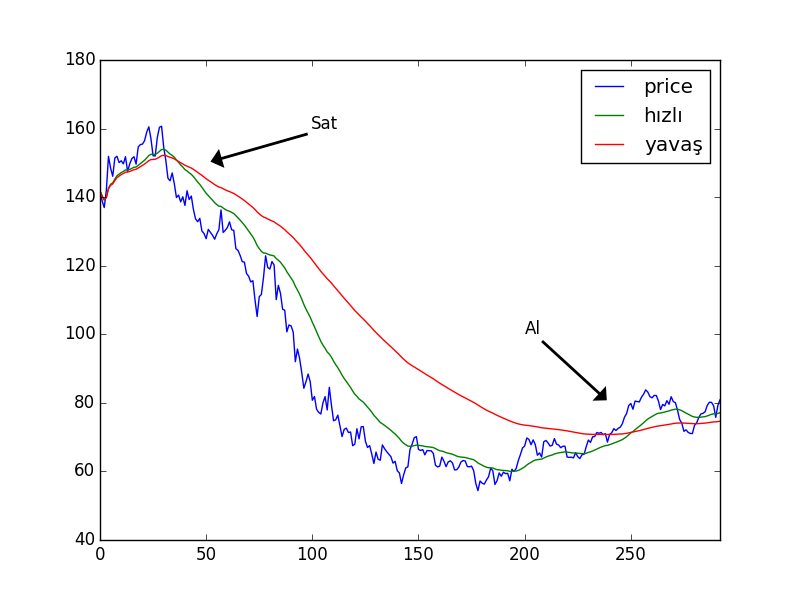
\includegraphics[height=6cm]{tser_mom_06.png}

Tabii alım ve satım olma / olmama türünden ikisel kararlar değil. [2] alımda
olma ve satıma olmayı sürekli bağlamda düşünüyor, yani üstteki örnekte hangi
``pozisyonda'' olunduğu hesabı için hızlı EWMAC'ten yavaş olan çıkartılıyor, ve
bu fark kadar, ki bir reel sayı, posiyona giriliyor. Eğer sonuç -4.5 ise 4.5
ünite kadar açığa satışta olmak lazım. 

Negatif Yamukluk (Negative Skew)

Momentum stratejilerinin, özelde EWMA stratejilerinin pozitif yamukluğu olduğu
hep söylenir. Böyle olup olmadığını kontrol edelim.

\begin{minted}[fontsize=\footnotesize]{python}
import sys; sys.path.append('../tser_voltar')
import util, pandas as pd, zipfile
f = 'CORN_price.csv'
with zipfile.ZipFile('../tser_voltar/legacycsv.zip', 'r') as z:
    df =  pd.read_csv(z.open(f),sep=',',index_col=0,parse_dates=True)
pred = util.ewma(df.PRICE,2,8)
print util.skew(df.PRICE, pred)
\end{minted}

\begin{verbatim}
1.18
\end{verbatim}

Daha ``yavaş'' EWMA stratejilerinde negatif yamukluk görülebilir, hızlı olanda
görülmüyor çünkü bu strateji daha hızlı adapte oluyor, [2]'nin tarif ettiği gibi
uzun zaman azar azar kaybedip düşüş veya çıkış başlayınca birdenbire kazanç
sağlıyor. 

Kaynaklar

[1] Chan, {\em Algorithmic Trading}

[2] Carver, {\em Systematics Trading}

\end{document}
